% multiple1902 <multiple1902@gmail.com>
% intro.tex
% Copyright 2011~2012, multiple1902 (Weisi Dai)
% https://code.google.com/p/xjtuthesis/
%
% It is strongly recommended that you read documentations located at
%   http://code.google.com/p/xjtuthesis/wiki/Landing?tm=6
% in advance of your compilation if you have not read them before.
%
% This work may be distributed and/or modified under the
% conditions of the LaTeX Project Public License, either version 1.3
% of this license or (at your option) any later version.
% The latest version of this license is in
%   http://www.latex-project.org/lppl.txt
% and version 1.3 or later is part of all distributions of LaTeX
% version 2005/12/01 or later.
%
% This work has the LPPL maintenance status `maintained'。
%
% The Current Maintainer of this work is Weisi Dai。
%

\chapter{基于边缘骨架切割的文字检测方法}
\echapter{Text detection based on Skeleton-cut detector}

    \section{问题的提出}
    \esection{Questions Posed}

    \section{方法原理与步骤}
    \esection{Principle and Summary of The Method}

    基于边缘骨架切割的文字检测子的具体流程如图\ref{fig.c31_overview}所示。首先对于输入的场景文字图片,利用结构化边缘检测方法\cite{Dollar2015Fast}得到输入图片的结构化边缘响应图,如图\ref{fig.c31_overview}(b) 所示。然后基于一系列像素强度值阈值,对边缘响应图进行分割,得到相应的二值化边缘图。接着在每个二值边缘图上,通过细化操作得到其边缘骨架图,如图\ref{fig.c31_overview}(c)所示。图中的红色结点是在边缘骨架上,通过8领域内像素点分析所找到的边缘骨架结点。而文字边缘与背景间的粘连点,就存在于这些边缘骨架结点中。
    为了将文字边缘从背景杂质中切割出来,需要切割开这些边缘骨架结点,以解决文字边缘的粘连问题。而由不同的二值边缘图所生成的边缘骨架图上的结点是不同的。因此选择合适的边缘骨架图上的结点进行切割,是解决文字边缘粘连问题的核心步骤。
    
    \begin{figure*}[htbp]
    \centering
    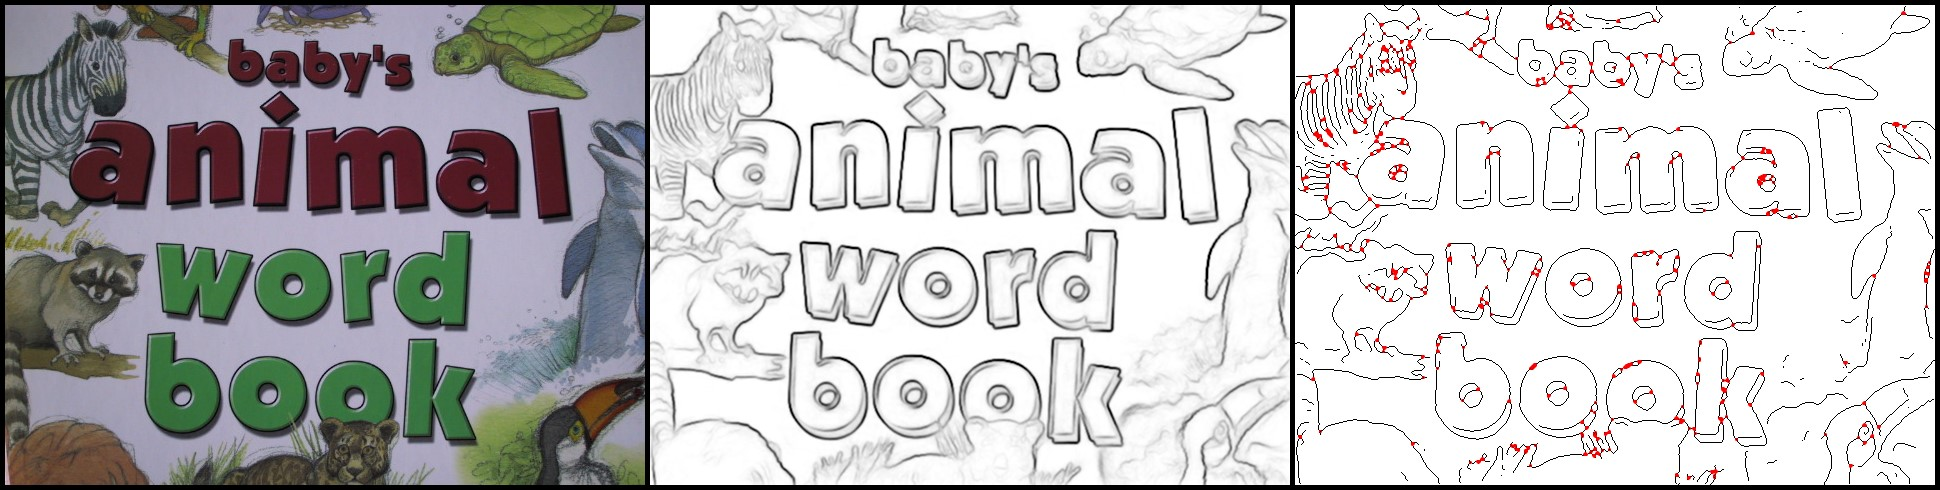
\includegraphics[width=\textwidth]{./figures/c31_overview_1.jpg}
    \begin{minipage}[t]{0.32\linewidth}
    \centerline{ \small (a)输入的场景文字图像}
    \end{minipage}
    \begin{minipage}[t]{0.32\linewidth}
    \centerline{ \small (b)场景文字图的边缘响应}
    \end{minipage}
    \begin{minipage}[t]{0.32\linewidth}
    \centerline{ \small (c)场景文字图的边缘骨架}
    \end{minipage}
    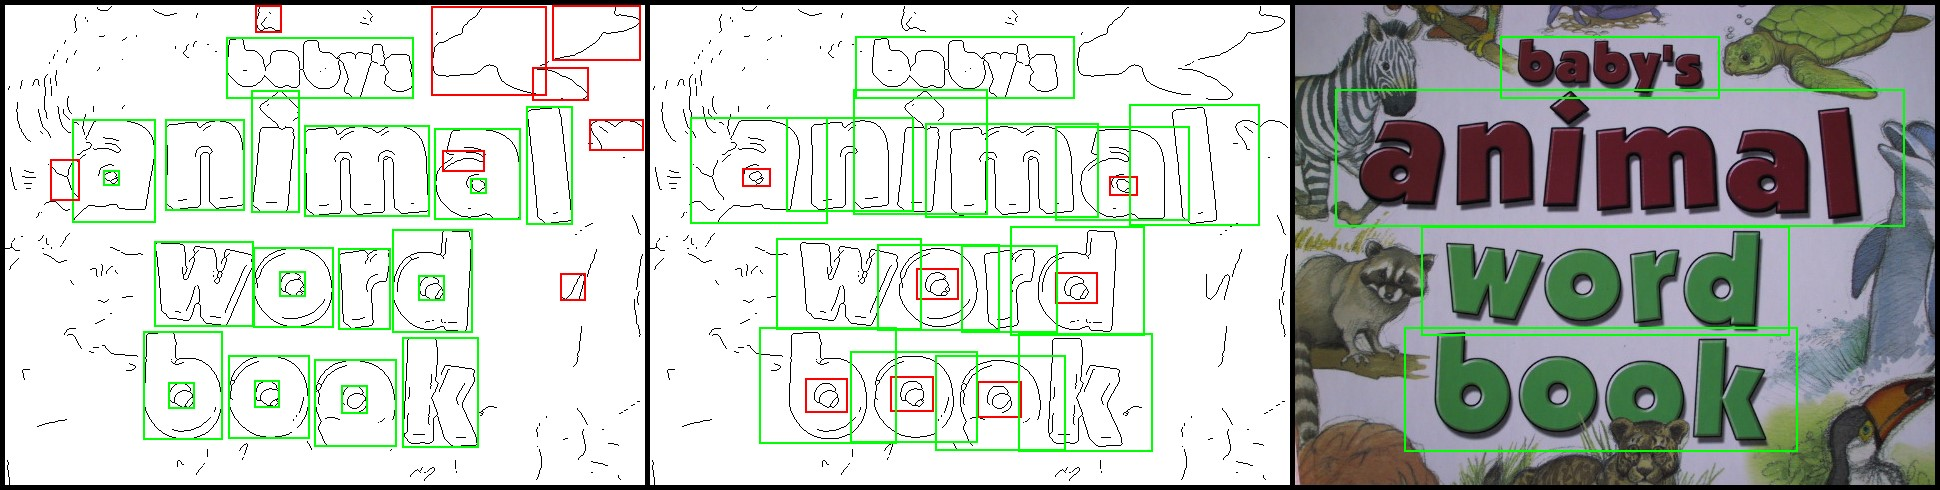
\includegraphics[width=\textwidth]{./figures/c31_overview_2.jpg}
    \begin{minipage}[t]{0.32\linewidth}
    \centerline{ \small (d)边缘骨架切割}
    \end{minipage}
    \begin{minipage}[t]{0.32\linewidth}
    \centerline{ \small (e)非文字边缘骨架图的滤除}
    \end{minipage}
    \begin{minipage}[t]{0.32\linewidth}
    \centerline{ \small (f)文字粗略定位结果}
    \end{minipage}
    \caption{基于边缘骨架切割的文字检测方法的流程图}
    \label{fig.c31_overview}
    \end{figure*}
    
    这里通过实验观察可知,那些分割阈值较低所得的二值边缘图所生成的边缘骨架较为杂乱,更可能是无效的边缘骨架,如图\ref{fig.c33_select_skeleton}(a)所示。   
    因此这里采用欧拉数计算,来从一系列边缘骨架图中选择出最合适的边缘骨架图,欧拉数的计算过程如图\ref{fig.c33_select_skeleton}(b) 所示。在边缘骨架图中,所有的候选边缘骨架都要经过形态学滤除,以过滤掉大部分明显不是文字的边缘骨架。该滤除过程如图\ref{fig.c31_overview}(c)到图\ref{fig.c31_overview}(d)的变化所示。紧接着,剩余的不易区分的非文字边缘骨架,可通过基于CNN的分类器来进一步滤除。该滤除过程如图\ref{fig.c31_overview}(d)到图\ref{fig.c31_overview}(e)所示,红色框中包含的不易区分的非文字边缘骨架,可通过CNN分类器去除掉。最后如图\ref{fig.c31_overview}(f)所示,基于非极大值抑制和文本行聚集操作,得到粗略的文本行定位结果。

    \section{文字骨架的提取与切割}
    \esection{Text skeleton's extraction and cutting}

        \subsection{文字骨架的生成}
        \esubsection{Text skeleton's construction}

        %一系列分割阈值,得到不同的二值边缘图,并生成相应的边缘骨架图;低分割阈值的二值图所生成骨架图较为杂乱,不适合用于后续的边缘骨架切割步骤;这部分内容在supplement上有,将其作图写在skeleton的生成一节中。

        \begin{figure*}[htbp]
        \centering
        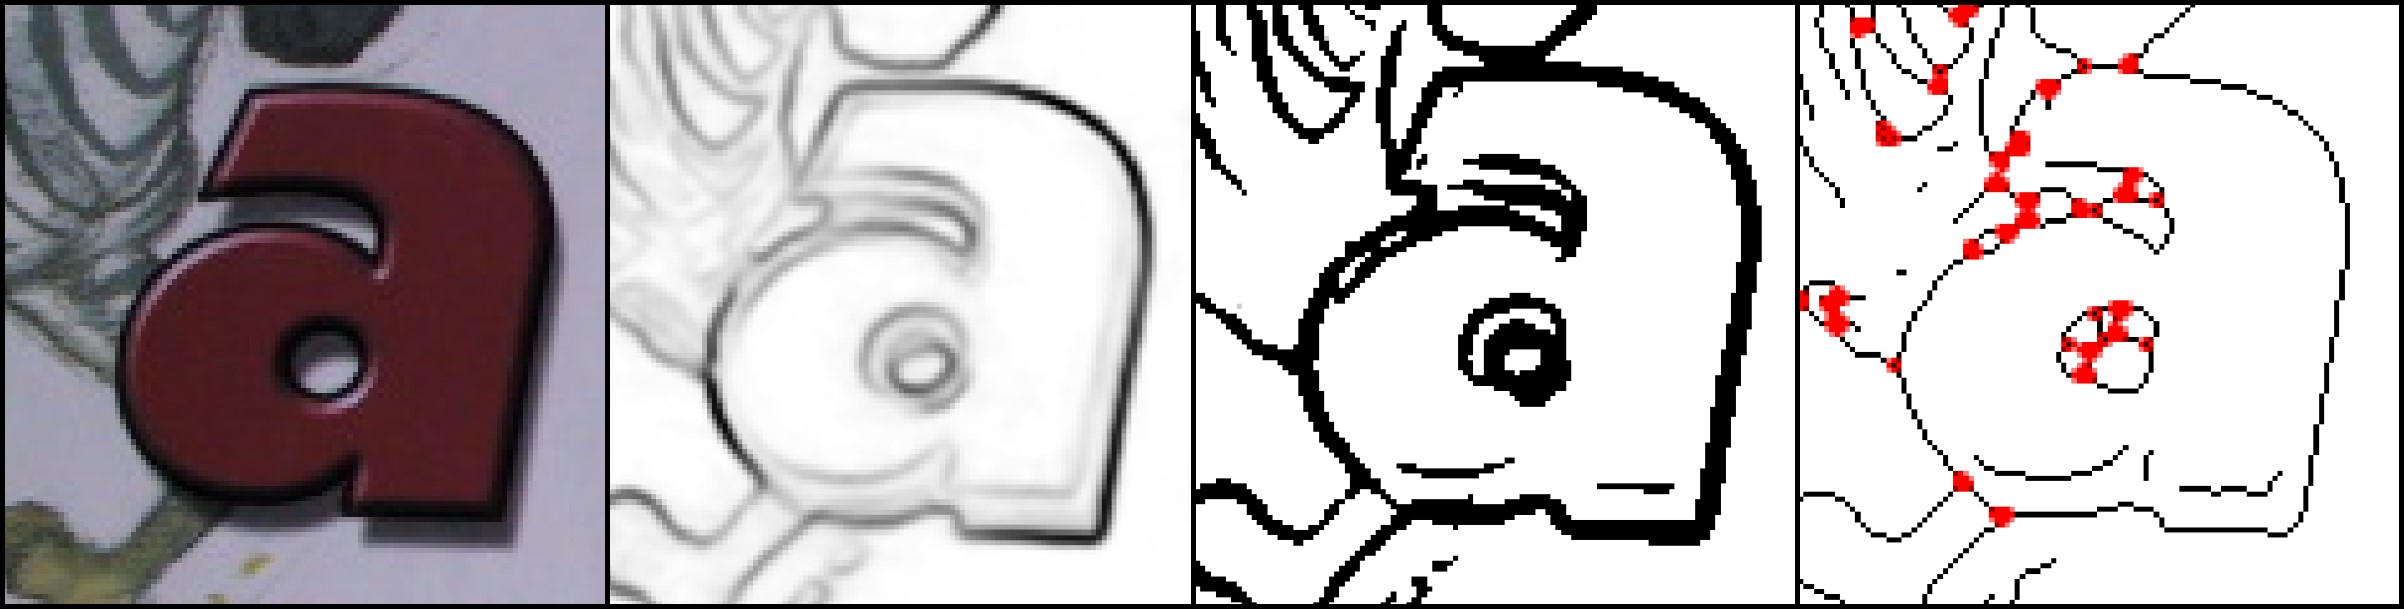
\includegraphics[width=\textwidth]{./figures/c32_skeleton.jpg}
        \begin{minipage}[t]{0.24\linewidth}
        \centerline{\small (a)原图}
        \end{minipage}
        \begin{minipage}[t]{0.24\linewidth}
        \centerline{\small (b)边缘响应}
        \end{minipage}
        \begin{minipage}[t]{0.24\linewidth}
        \centerline{\small(c)边缘二值图}
        \end{minipage}
        \begin{minipage}[t]{0.24\linewidth}
        \centerline{\small (d)边缘骨架图}
        \end{minipage}
        \caption{文字边缘骨架生成的流程图}
        \label{fig.c32_skeleton}
        \end{figure*}

        \subsection{文字骨架粘连点的检测和切割}
        \esubsection{Text adhesion-junctions' detection and cutting}

        \begin{figure}[htbp]
        \centering
        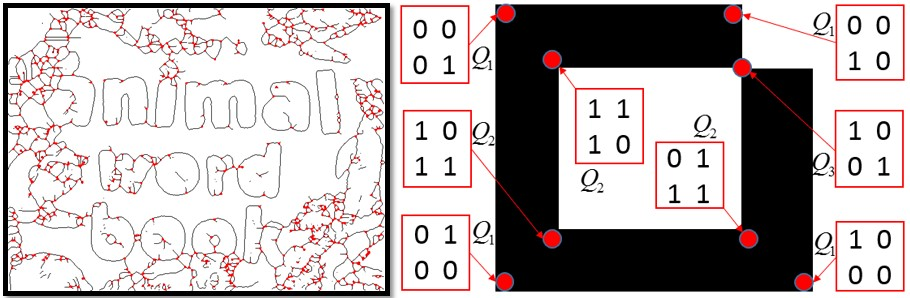
\includegraphics[width=\textwidth]{./figures/c33_select_skeleton.jpg}
        \begin{minipage}[t]{0.48\linewidth}
        \centerline{\small (a)无效的边缘骨架图}
        \end{minipage}
        \begin{minipage}[t]{0.48\linewidth}
        \centerline{\small (b)在边缘骨架图上计算欧拉数}
        \end{minipage}
        \caption{通过欧拉数的计算,选择出最合适的边缘骨架图}
        \label{fig.c33_select_skeleton}
        \end{figure}

    \section{非文字骨架的滤除}
    \esection{Non-text skeleton's filtering}

        \subsection{形态学滤除}
        \esubsection{Morphological filtering}

        \subsection{基于卷积神经网络的滤除}
        \esubsection{convolutional neural network-based filtering}

    \section{文本行生成}
    \esection{Text line's construction}

        \subsection{最稳定极值区域的提取}
        \esubsection{Extraction of the most stable extremum region}

        \subsection{文本行的局部迭代优化}
        \esubsection{Text line's iteratively local refinement}

    \section{实验和结果分析}
    \esection{Experimental Results}

        \subsection{实验数据集与评价标准}
        \esubsection{Data-set and Evaluation Protocol}

        \subsection{实验结果与分析}
        \esubsection{Experimental Results and Analysis}

    \section{本章小结}
    \esection{Brief Summary}


